\ifdefined\SPsubmission
\documentclass[review,11pt,a4paper]{elsarticle}
\usepackage{amsmath,amssymb,amsthm,array,booktabs,graphicx,float}
\usepackage[expansion=false]{microtype}
\usepackage{hyperref}
\usepackage{lineno}
\graphicspath{{../}}
\journal{Signal Processing}
\else
\documentclass[11pt]{article}
\usepackage[a4paper,margin=2.5cm]{geometry}
\usepackage{amsmath,amssymb,amsthm,array,booktabs,graphicx,microtype,float}
\usepackage[numbers]{natbib}
\usepackage{hyperref}
\fi
\usepackage{lmodern}
\hypersetup{hidelinks}
\ifdefined\SPsubmission
\renewcommand{\bibfont}{\fontsize{9}{10.5}\selectfont}
\setlength{\emergencystretch}{1em}
\else
\renewcommand{\bibfont}{\footnotesize}
\fi
\floatstyle{ruled}
\newfloat{algorithm}{tbp}{loa}
\floatname{algorithm}{Algorithm}

\newtheorem{theorem}{Theorem}
\newtheorem{proposition}{Proposition}
\newtheorem{corollary}{Corollary}
\newtheorem{lemma}{Lemma}
\newtheorem{remark}{Remark}

\newcommand{\HCRDtitle}{Hierarchical Convexity-Run Decomposition:
Finite-Sample Chord-Lobe Recovery and Interpretable LC--MS Transfer}
\newcommand{\HCRDabstract}{%
We introduce Hierarchical Convexity-Run Decomposition (HCRD), a finite
nonlinear transform that replaces runs of one discrete-curvature sign by
endpoint chords and recurses on retained knots.  Its signed residuals form an
exactly reconstructing, interpretable lobe hierarchy with linear total
knot-only work.  On an explicit alternating chord-lobe class under Gaussian
noise, we prove first-level boundary and component recovery, including
approximate sampled joins: if active curvature $\gamma$, join departure $\eta$,
and the simultaneous noise threshold $\tau$ satisfy
$\gamma>\eta+2\tau$, every boundary is recovered with probability at least
$1-\delta$.  Across 206,000 simulated signals, zero failures were observed
among 80,000 draws in the strict certified regions.  Structural results
establish finite termination, affine equivariance, variation control, global
discontinuity of the hard map, and stable companions.  In frozen no-refit
transfers between two fully labelled LC--MS studies, HCRD-8 plus an
independently reimplemented quality score improved average precision by
0.1181 and 0.1005.  An equal-dimensional Gaussian-derivative control tied HCRD
in one direction, whereas HCRD was superior in the reverse; a larger
TARDIS/FAME shift did not confirm superiority.  HCRD therefore provides a
simple morphological inductive bias with a quantitative recovery regime and
explicit application boundaries.}
\ifdefined\SPsubmission
\else
\title{\HCRDtitle}
\author{Saveliy Baturin\\Independent Researcher}
\date{Draft \today}
\fi

\begin{document}
\ifdefined\SPsubmission
\begin{frontmatter}
\title{\HCRDtitle}
\author[1]{Saveliy Baturin}
\address[1]{Independent Researcher}
\begin{abstract}
\HCRDabstract
\end{abstract}
\begin{keyword}
discrete curvature \sep nonlinear decomposition \sep hierarchical
representation \sep finite-sample recovery \sep LC--MS \sep waveform morphology
\end{keyword}
\end{frontmatter}
\modulolinenumbers[5]
\linenumbers
\else
\maketitle

\begin{abstract}
\HCRDabstract
\end{abstract}
\fi

\section{Introduction}
Empirical mode decomposition (EMD) motivated data-adaptive analysis of
nonstationary signals through extrema and envelope sifting
\citep{huang1998emd}.  Intrinsic time-scale decomposition (ITD) subsequently
introduced an efficient iterative baseline--rotation construction based on
piecewise-linear transformations between extrema \citep{frei2006itdpatent,frei2007itd}.
In particular, its patent measures a lobe height from an extremum to the line
joining neighbouring extrema and recursively decomposes the concatenated
baseline.  Thus straight-line lobe geometry and recursive piecewise-linear
baselines are prior art.  The method studied here arose independently from a
different selection and update rule: partition a sampled graph into maximal
runs of one divided-curvature sign, replace each entire run by its endpoint
chord, and allow only the retained knots at the next level.
Figure~\ref{fig:method} previews the resulting curvature-run split, endpoint
chords, and exact two-level synthesis.

The primitive is related to inflection-point sampling \citep{iem2014inflection},
but iteration produces a nested, exactly reconstructing hierarchy.  More
directly, the PDE sifting construction of Del\'echelle et al.
\citep{delechelle2005pde} converges to a piecewise-cubic interpolant through
successive inflection points, while the $\alpha$-shape construction of Chessel
et al. \citep{chessel2009alpha} defines a
convexity-driven geometric scale space.  Recent EMD software also includes
inflection-point interpolation as one of several local-mean estimators
\citep{vanjaarsveldt2023advemdpy}, and special-inflection-point EMD augments
extrema with inflections from the signal and its derivatives
\citep{kafil2023sipemd}.  These works preclude treating the use of inflection
points itself as novel.  HCRD differs in using a one-pass discrete
curvature-sign walk, endpoint chords, and recursively nested eligible knot
sets, rather than auxiliary envelope knots, PDE evolution, $\alpha$-shape
subsampling, or repeated IMF sifting.

The closest theoretical comparison classes further include Gaussian scale
space \citep{babaud1986scale}, $\ell_1$ trend filtering
\citep{kim2009trend}, iterative filtering \citep{lin2009iterative}, connected
operators represented by region trees \citep{salembier1998connected}, and the
LULU discrete pulse transform and its linear-time one-dimensional Roadmaker
construction \citep{anguelov2010lulu,laurie2011roadmaker}.  Connected operators
prune flat-zone region trees, while DPT produces constant block pulses on
connected supports; neither uses affine residual lobes from the HCRD
curvature-run knot tree.  HCRD's contribution is the particular finite discrete
operator and the combination of hierarchy, reconstruction,
geometric sign, stability, limitation, and calibrated-inference results---not
the generic idea of using curvature, inflection points, chord lobes, or a
nonlinear component hierarchy.

Table~\ref{tab:method-comparison} makes the closest distinctions explicit.
ITD is the nearest chord-baseline recursion and DPT the nearest exact nonlinear
pulse hierarchy; neither uses curvature-run knot selection.  Trend filtering
instead solves a stable penalized optimization problem.

\begin{table}[t]
\centering
\caption{Closest one-dimensional representations.  ``Exact'' means that the
native components plus the final baseline reconstruct the input; costs are
nominal.}
\label{tab:method-comparison}
\footnotesize
\setlength{\tabcolsep}{5pt}
\renewcommand{\arraystretch}{1.08}
\begin{tabular}{@{}>{\raggedright\arraybackslash}p{0.14\linewidth}
                    >{\raggedright\arraybackslash}p{0.255\linewidth}
                    >{\raggedright\arraybackslash}p{0.245\linewidth}
                    >{\raggedright\arraybackslash}p{0.25\linewidth}@{}}
\toprule
Method & Primitive and native components & Reconstruction / hierarchy & Computation and regularity \\
\midrule
HCRD & Curvature-sign runs; endpoint-chord residual lobes
     & Exact; nested knot subsets
     & $O(n)$ total sparse; hard decisions; irregular $x$ \\
ITD \citep{frei2007itd} & Extrema updates; linear baseline and rotations
     & Exact; recursive baseline
     & $O(n)$ per level; hard extrema; ordered grid \\
LULU/DPT \citep{anguelov2010lulu,laurie2011roadmaker}
     & Order / flat zones; constant pulses
     & Exact; size hierarchy
     & $O(n)$ Roadmaker; order-based sequence \\
RDP \citep{douglas1973reduction}
     & Maximum chord error; polygonal approximation
     & Exact with residual; split tree
     & $O(n^2)$ worst case; hard ties; arbitrary coordinates \\
$\ell_1$ trend filtering \citep{kim2009trend}
     & Penalized curvature; piecewise-linear fit
     & Exact with residual; no native hierarchy
     & Convex optimization; continuous fit; irregular variants \\
Gaussian scale space \citep{babaud1986scale}
     & Convolution scale; smoothed signals
     & Scale differences; scale-ordered
     & FFT / direct; continuous; regular-grid standard \\
\bottomrule
\end{tabular}
\end{table}

The LC--MS use case is also distinct from end-to-end peak picking.  PeakBot
detects local maxima and classifies two-dimensional chromatographic regions
with a convolutional network \citep{bueschl2022peakbot}; PeakDetective combines
an autoencoder with active learning for dataset-specific curation
\citep{stancliffe2023peakdetective}; TMSQE learns targeted peak-quality
embeddings \citep{yang2024tmsqe}; and MassCube integrates feature detection,
evaluation, grouping, and annotation \citep{yu2025masscube}.  HCRD instead
supplies transparent features for already bounded one-dimensional EICs and is
tested here under no-target-refit transfer.  These systems therefore define the
application landscape but are not interchangeable baselines for the present
fixed-box question.

\begin{figure}[H]
\centering

\includegraphics[width=\linewidth]{figures/method_overview.pdf}
\caption{Two explicit HCRD steps on a synthetic EIC-like graph.  Curvature-sign
changes delimit retained knots.  Replacing every level-1 run by its endpoint
chord gives baseline $b^1$ and signed residual $d^1$; applying the same
operation to $b^1$ gives $b^2$ and $d^2$.  The displayed truncation reconstructs
$y=b^2+d^2+d^1$ exactly, and recursion may continue.  Shaded lobes can be
summarised by area or energy, but the decomposition is the complete residual
shape.  This computed example illustrates the operator; it is not a stability
proof and levels are not asserted to be frequency bands.}
\label{fig:method}
\end{figure}

Our contributions are:
\begin{enumerate}
  \item a complete finite algorithm for the centred curvature-run operator,
        with nested-hierarchy, exact-reconstruction, sparse linear-work, affine,
        variation, and interpretable lobe-shape results;
  \item an HCRD-specific finite-sample recovery theorem for an explicit
        alternating chord-lobe class with exact or approximate sampled joins,
        local and stochastic hierarchy-agreement guarantees, and theorem-linked
        phase experiments over 206,000 signals;
  \item a sharp global discontinuity boundary together with stable proximal
        and persistence companions;
  \item frozen cross-study LC--MS validation, multilevel and area ablations,
        a matched-capacity conventional control, operational review-queue
        analysis, implementation and refitting sensitivities, and external
        limitation studies.  Optional scan and post-selection theory is given
        in the supplement.
\end{enumerate}

\section{Definition of the transform}
Let $x_0<\cdots<x_{n-1}$ and $y=(y_0,\ldots,y_{n-1})\in\mathbb R^n$.
Define divided slopes and discrete curvatures by
\begin{equation}
s_i(y)=\frac{y_{i+1}-y_i}{x_{i+1}-x_i},\qquad
\kappa_i(y)=s_i(y)-s_{i-1}(y).
\end{equation}
For absolute and relative tolerances $a,r\ge0$, define
\begin{equation}
 \tau=a+r\max\{1,\max_i|s_i(y)|\}.
\end{equation}
A curvature is active when $|\kappa_i|>\tau$ and inactive otherwise.  The
mathematical hard operator uses $a=r=0$; the implementation defaults to a tiny
relative tolerance to suppress floating-point curvature on interpolated affine
segments. Algorithm~\ref{alg:hcrd} specifies every branch of the centred rule.

\begin{algorithm}[H]
\caption{One centred HCRD hierarchy on an irregular grid}
\label{alg:hcrd}
\small
\textbf{Input:} strictly increasing $x$, samples $y$, tolerances $a,r\ge0$,
and optional depth cap $L$.  Initially $E=(0,\ldots,n-1)$.
\begin{enumerate}
\setlength{\itemsep}{1pt}
\item On the current eligible list $E=(e_0,\ldots,e_{m-1})$, set
$z_i=y_{e_i}$, $u_i=x_{e_i}$, compute divided curvatures, and compute $\tau$
from the current divided slopes.  If $m=2$, stop.
\item Set the local start $p=0$ and the new local knot list $K=(0)$.
\item Let $f$ be the first active curvature index in
$\{p+1,\ldots,m-2\}$.  If none exists, append $m-1$ to $K$ and finish this
level.  Otherwise set the active sign to $\operatorname{sign}(\kappa_f)$,
$\ell=f$, and scan right.
\item Ignore inactive curvatures.  On each active curvature of the same sign,
update $\ell$.  Let $q$ be the first active curvature of the opposite sign.  If
no such $q$ exists, append $m-1$ and finish the level.
\item If $q-\ell=2$, the single inactive curvature at $\ell+1$ is the sampled
transition and the candidate is $c=\ell+1$.  At zero tolerance this is exactly
the sampled-zero case.
\item Otherwise set $c=\ell$ only when
$|\kappa_\ell|<|\kappa_q|$ and $\ell\ne f$; set $c=q$ in every other case.
Thus equal magnitudes are tied to the right, first-opposite side, and a long
inactive plateau never creates an interior knot.
\item Enforce strict coarsening by replacing
$c$ with $\max\{p+2,\min(c,m-1)\}$.  Append $c$ to $K$, set $p=c$, and return
to step 3.  The final remainder always closes at $m-1$.
\item Map the local knots back to original indices, $E'=(e_k:k\in K)$.
Interpolate the endpoint chords through $(x_i,y_i)$ for $i\in E'$ to obtain the
next baseline; subtract it to obtain the signed detail.
\item Set $E\leftarrow E'$ and repeat until $|E|=2$ or the optional cap $L$ is
reached.  Later levels therefore use only previously retained knots.
\end{enumerate}
\end{algorithm}

Let $K(y)$ denote the first mapped knot set and let $Ty$ be linear
interpolation through $(x_k,y_k)$ for $k\in K(y)$.

Set $b^0=y$ and recursively define
\begin{equation}
b^{j+1}=Tb^j,\qquad d^{j+1}=b^j-b^{j+1}.
\end{equation}
The implementation restricts eligible knots at level $j+1$ to knots retained
at level $j$.  This prevents the insertion of geometrically redundant samples
inside an existing affine segment.
In local eligible-knot coordinates, a nonterminal centred interval is required
to advance by at least two old intervals; the first-opposite and sampled-zero
cases below satisfy this convention explicitly.

\section{Structural results}
\begin{theorem}[Exact reconstruction]
For every computed level $J$,
\begin{equation}
y=\sum_{j=1}^{J}d^j+b^J.
\end{equation}
\end{theorem}
\begin{proof}
Substitute $d^j=b^{j-1}-b^j$ and telescope.
\end{proof}

\begin{theorem}[Finite nested hierarchy]
\label{thm:finite}
The eligible knot sets are nested.  Every nonterminal HCRD interval consumes at
least two intervals of the preceding level.  Consequently the hierarchy ends
at the endpoint chord after at most
$\max\{1,\lceil\log_2(n-1)\rceil\}$ implemented levels.
\end{theorem}
\begin{proof}
Eligibility gives nesting.  A run can close only after the walk has passed the
first active old curvature and reached either an eligible intervening zero or
the first active curvature of opposite sign.  Thus an old interior knot is
removed in each nonterminal new interval.  Pairing old intervals gives the
halving recurrence, with at most one terminal remainder.
\end{proof}

\begin{corollary}[Linear-work knot-only hierarchy]
\label{cor:sparse}
Let $N_0=n-1$ and let $N_j$ be the number of intervals after level $j$.
An implementation that scans only the current eligible knot list has $O(n)$
total knot-walk work and stores
\begin{equation}
\sum_{j=1}^{J}|K_j|<2(n-1)+J=O(n).
\end{equation}
Dense length-$n$ baselines and details can be reconstructed exactly on demand.
\end{corollary}
\begin{proof}
The halving recurrence gives $N_j\le\lceil N_0/2^j\rceil$ and
$J=O(\log n)$.  For integer $N_0\ge1$,
$\lceil N_0/2^j\rceil\le (N_0-1)/2^j+1$; hence
$\sum_{j=1}^J N_j<N_0-1+J\le2N_0$.  Since $|K_j|=N_j+1$, the displayed
finite bound follows.  The analogous series beginning with $N_0$ bounds the
total scanned eligible intervals by $O(n)$.  Chord interpolation through each
stored knot set reproduces the dense baseline, and adjacent differences
reproduce the details.
\end{proof}

\begin{proposition}[Signed structures]
On a discretely convex run, $y-Ty\le0$.  On a discretely concave run,
$y-Ty\ge0$.
\end{proposition}
\begin{proof}
A convex polygonal graph lies below its endpoint secant.  Reverse the inequality
for a concave graph.
\end{proof}

For structure $r$ of detail $d^j$ on $I_{jr}=[x_a,x_b]$, define its signed
area, geometric mass, and quadratic residual energy by
\begin{equation}
S_{jr}=\int_{I_{jr}}d^j(x)\,dx,\qquad
A_{jr}=\int_{I_{jr}}|d^j(x)|\,dx,\qquad
E_{jr}=\int_{I_{jr}}d^j(x)^2\,dx,
\label{eq:geometric-mass}
\end{equation}
where $d^j$ is the exact piecewise-linear interpolant of the sampled residual.
These quantities are computable from retained knots without materializing a
length-$n$ detail.  Signed structures give $A_{jr}=|S_{jr}|$.  Under
$y\mapsto cy+\alpha+\beta x$, $A_{jr}$ scales by $|c|$ and $E_{jr}$ by $c^2$;
under an orientation-preserving horizontal affine change
$x\mapsto\rho x+\tau$, both integrals acquire the Jacobian factor $\rho$.
Thus $A_{jr}$ is a literal morphology measure in signal-units times
coordinate-units.  It is not spectral energy, and the nonorthogonal hierarchy
has no Parseval identity.

\begin{proposition}[Dimensionless lobe shape]
For a nonzero structure let $W=x_b-x_a$, $H=\max_{I_{jr}}|d^j|$, and define
\begin{equation}
 F=\frac{A_{jr}}{WH},\qquad
 C=\frac{A_{jr}^2}{W E_{jr}}.
\end{equation}
Then $0<F\le1$ and $0<C\le1$.  Both are invariant under nonzero vertical
scaling, affine trend addition, and orientation-preserving horizontal affine
changes.  A piecewise-linear triangular lobe has $(F,C)=(1/2,3/4)$ regardless
of apex location; a parabolic lobe $4Ht(W-t)/W^2$ has
$(F,C)=(2/3,5/6)$.
\end{proposition}
\begin{proof}
$A\le WH$ follows from $|d|\le H$, while Cauchy--Schwarz gives
$A^2\le WE$.  The scaling laws above cancel in both ratios.  Direct integration
gives the two examples.
\end{proof}

The first ratio is the implemented per-structure shape factor.  The second is
available as a quadratic concentration descriptor but was not added after the
LC--MS protocols were frozen.  Keeping $A_{jr}$ or either invariant for each
moving support and level also yields a low-dimensional temporal morphology
series; collapsing all structures to one total mass discards that evolution.

\begin{theorem}[Affine equivariance]
For zero curvature tolerance, nonzero $a$, and
$\ell_i=\alpha+\beta x_i$,
\begin{equation}
T(ay+\ell)=aTy+\ell.
\end{equation}
Hence every HCRD detail is invariant to affine trend addition and scales by
$a$.
\end{theorem}
\begin{proof}
Affine addition cancels from adjacent divided-slope differences.  Multiplication
by $a$ preserves all transition locations, although negative $a$ reverses the
signs.  Chord interpolation commutes with both operations.
\end{proof}

\begin{theorem}[Range and total variation]
For one HCRD step,
\begin{equation}
\min y\le (Ty)_i\le\max y,\qquad TV(Ty)\le TV(y).
\end{equation}
\end{theorem}
\begin{proof}
Every chord sample is a convex combination of its endpoint values.  Its
variation equals the absolute difference between the endpoint values, which is
no greater than the variation of the removed polygonal subpath.
\end{proof}

\section{Stability and its obstruction}
\begin{theorem}[Stability inside a curvature-decision cell]
\label{thm:local-stability}
On a unit grid suppose $\gamma=\min_i|\Delta^2y_i|>0$ and let
\begin{equation}
\eta=\min_{\Delta^2y_i\Delta^2y_{i+1}<0}
\bigl||\Delta^2y_i|-|\Delta^2y_{i+1}|\bigr|,
\end{equation}
with $\eta=+\infty$ if there is no sign transition.  For the centred rule, if
$\|e\|_\infty<\min\{\gamma/4,\eta/8\}$, then $K(y+e)=K(y)$ and
\begin{align}
\|T(y+e)-Ty\|_\infty &\le \|e\|_\infty,\\
\|(I-T)(y+e)-(I-T)y\|_\infty &\le 2\|e\|_\infty.
\end{align}
\end{theorem}
\begin{proof}
The coefficient norm of the second-difference stencil $(1,-2,1)$ is four, so
the first margin prevents a curvature-sign change.  A difference of two
absolute curvature magnitudes moves by at most $8\|e\|_\infty$, so the second
margin preserves every centred transition comparison.  The knot walk is
therefore fixed.  Fixed-knot interpolation is a convex combination of endpoint
perturbations, and the detail estimate follows by the triangle inequality.
\end{proof}

The second margin is necessary: $(0,0,1,3,4)$ has curvatures $(1,1,-1)$,
whereas $(0,0,1,3-\varepsilon,4-2\varepsilon)$ has the same signs but selects
the other side of the tied centred transition.  The legacy first-opposite rule
does not compare magnitudes and requires only the sign margin.

\begin{proposition}[Global discontinuity]
The raw HCRD baseline operator is not globally continuous.
\end{proposition}
\begin{proof}
For $y^\pm=(-2,0,2\pm\varepsilon,-2)$, the inputs approach one another as
$\varepsilon\downarrow0$, whereas one first baseline retains the interior peak
and the other becomes the constant endpoint chord.  Their sup-norm separation
tends to four.
\end{proof}

\begin{theorem}[No continuous generic-agreement extension]
\label{thm:impossibility}
For four-sample signals let
$G=\{y:\min_i|\Delta^2y_i|>0\}$.  There is no globally continuous map
$F:\mathbb R^4\to\mathbb R^4$ that agrees with the raw HCRD baseline $T$ on
all of $G$.
\end{theorem}
\begin{proof}
For every $0<\varepsilon<1$, both
$y^\pm_\varepsilon=(-2,0,2\pm\varepsilon,-2)$ lie in $G$ and converge to the
same $y^0$.  Agreement on $G$ makes $F(y^\pm_\varepsilon)$ equal the two HCRD
outputs in the preceding counterexample, whose limits are separated by four.
Continuity at $y^0$ would force both limits to equal $F(y^0)$, a contradiction.
\end{proof}

\begin{remark}
HCRD is not an orthogonal transform and need not contract Euclidean energy.  For
$y=(-2,-1,-2)$, one has $Ty=(-2,-2,-2)$ and $\|Ty\|_2>\|y\|_2$.
\end{remark}

\ifdefined\SPsubmission
\section{Stable companion representations}
Hard knot decisions are locally stable inside a curvature-decision cell but
cannot be made globally continuous.  Two complementary summaries retain
interpretability while giving global perturbation control.  First, for the
divided-curvature matrix $D$ and a proper closed convex function $\phi$, define
\begin{equation}
P_\phi y=\mathop{\rm argmin}_z
\left\{\frac12\|y-z\|_2^2+\phi(Dz)\right\},\qquad Q_\phi=I-P_\phi .
\end{equation}
The implemented choices are the established $\ell_1$ trend penalty and a
quadratic curvature penalty; their role is to provide a stable outer split,
not a new convex estimator.

\begin{theorem}[Exact globally nonexpansive outer split]
\label{thm:prox}
Both $P_\phi$ and $Q_\phi$ are firmly nonexpansive, $y=P_\phi y+Q_\phi y$, and
the split is equivariant to addition of every affine sequence in $\ker D$.
\end{theorem}

\begin{corollary}[Irregular-grid sign certificate]
If $\|e\|_2\le\rho$ and $h_i=x_{i+1}-x_i$, the $i$th guide curvature changes
by at most $2\rho(h_{i-1}^{-1}+h_i^{-1})$; guide curvatures above this bound
therefore have certified sign.
\end{corollary}

Second, let $u_y^+=(D_xy)_+$ and $u_y^-=(-D_xy)_+$ on the interior-index path.
The bottleneck distances between the two signed zero-dimensional superlevel
diagrams, including the essential birth heights, define a pullback
pseudometric $d_{\rm SC}$ on signals.  Equal summaries, rather than only
affine differences, form its zero-distance classes.

\begin{theorem}[Global signed-curvature persistence stability]
\label{thm:persistence}
For two signals on the same irregular grid,
\begin{equation}
d_{\rm SC}(y,z)\le C_x\|y-z\|_\infty,
\qquad C_x=2\max_i\{h_{i-1}^{-1}+h_i^{-1}\}.
\end{equation}
A finite signed-curvature bar with lifetime greater than
$2C_x\|y-z\|_\infty$ cannot disappear into the diagonal.
\end{theorem}

\begin{proposition}[Curvature visibility limit]
If $y(t)=g(t)+a\sin(\omega t)$ and
$g''(t)>|a|\omega^2$ on an interval, then $y''$ has one sign there; a raw
inflection-run rule cannot isolate the oscillation on that interval.
\end{proposition}

Complete definitions, proofs, and numerical stability audits are given in the
supplement.
\else
\section{A stable proximal companion}
Let $D$ be the divided-curvature matrix and let $\phi$ be a proper closed
convex function.  Define
\begin{equation}
P_\phi y=\mathop{\rm argmin}_z
\left\{\frac12\|y-z\|_2^2+\phi(Dz)\right\},\qquad
Q_\phi=I-P_\phi .
\end{equation}
We implement the established $\ell_1$ trend penalty
$\phi(u)=\lambda\|u\|_1$ \citep{kim2009trend} and a quadratic curvature
penalty $\phi(u)=\lambda\|u\|_2^2/2$.  These guide operators themselves are
not claimed as novel; their role is to give HCRD an exact stable outer split.

\begin{theorem}[Exact globally nonexpansive outer split]
\label{thm:prox}
Both $P_\phi$ and $Q_\phi$ are firmly nonexpansive and
\begin{equation}
y=P_\phi y+Q_\phi y.
\end{equation}
Moreover, if $D\ell=0$, then
$P_\phi(y+\ell)=P_\phi y+\ell$ and $Q_\phi(y+\ell)=Q_\phi y$.
\end{theorem}
\begin{proof}
The divided-curvature matrix has full row rank, so properness of $\phi$ makes
$\phi\circ D$ proper.  The objective is coercive and strongly convex, hence has
a unique minimizer.  The standard
proximal-map theorem and Moreau decomposition make a proximal map and its
residual firmly nonexpansive \citep{parikh2014proximal}.  Exact splitting is
the definition of $Q_\phi$.  Translating both $y$ and the candidate minimizer
by $\ell\in\ker D$ leaves the objective unchanged.
\end{proof}

\begin{corollary}[Irregular-grid sign certificate]
Suppose $\|e\|_2\le\rho$ and put $h_{i-1}=x_i-x_{i-1}$ and
$h_i=x_{i+1}-x_i$.  The $i$th guide curvature changes by at most
\begin{equation}
c_i\rho=2\rho(h_{i-1}^{-1}+h_i^{-1}).
\end{equation}
Thus every guide curvature satisfying
$|\kappa_i(P_\phi y)|>c_i\rho$ has a fixed sign throughout the input ball.
Other curvatures must be marked uncertified.
\end{corollary}
\begin{proof}
Theorem~\ref{thm:prox} bounds the guide perturbation in $\ell_2$, hence also
coordinatewise, by $\rho$.  The absolute coefficient sum of the irregular
three-point curvature row is $2(h_{i-1}^{-1}+h_i^{-1})$.
\end{proof}

We retain $Q_\phi y$ explicitly and apply HCRD only to the guide $P_\phi y$,
so the complete representation still reconstructs $y$.  Theorem~\ref{thm:prox}
applies to the outer split, not to the hard knot hierarchy.  Indeed,
Theorem~\ref{thm:impossibility} rules out global continuity for any hard
replacement that preserves every generic raw decision.

\subsection{Stable signed-curvature persistence}
Hard knot locations are not the only possible summary of the curvature walk.
Let $P$ be the path on the $n-2$ interior sample indices and define the
nonnegative vertex functions
\begin{equation}
u_y^+=(D_xy)_+,\qquad u_y^-=(-D_xy)_+.
\end{equation}
Extend them linearly over the path edges.  For a nonnegative function $u$, let
$\mathcal D_0^{\rm fin}(u)$ be the finite part of its ordinary zero-dimensional
superlevel persistence diagram and let $M(u)=\max u$ record the birth of its
unique essential component.  Define
\begin{align}
d_{\rm SC}(y,z)=\max\{&d_B(\mathcal D_0^{\rm fin}(u_y^+),
                              \mathcal D_0^{\rm fin}(u_z^+)),
|M(u_y^+)-M(u_z^+)|,\nonumber\\
&d_B(\mathcal D_0^{\rm fin}(u_y^-),
     \mathcal D_0^{\rm fin}(u_z^-)),
|M(u_y^-)-M(u_z^-)|\}.
\end{align}
This is the pullback of a metric on the signed persistence summaries and is
therefore a pseudometric on signals.  It becomes a metric on the quotient
$y\sim z$ if and only if their two finite diagrams and two essential birth
heights agree.  Quotienting only by affine functions is insufficient: on a
unit grid, $y=(0,0,1,2,5)$ and $z=(0,0,2,4,7)$ have positive curvatures
$(1,0,2)$ and $(2,0,1)$, hence identical summaries by path reflection and
$d_{\rm SC}(y,z)=0$, although $z-y$ is not affine.

\begin{theorem}[Global signed-curvature persistence stability]
\label{thm:persistence}
For two signals on the same irregular grid,
\begin{equation}
d_{\rm SC}(y,z)\le C_x\|y-z\|_\infty,
\qquad
C_x=2\max_i\{h_{i-1}^{-1}+h_i^{-1}\}.
\end{equation}
If $\|y-z\|_\infty\le\varepsilon$, every finite bar of either sign with
lifetime greater than $2C_x\varepsilon$ has a finite same-sign match for the
other signal.
\end{theorem}
\begin{proof}
The absolute row sum of $D_x$ is
$2(h_{i-1}^{-1}+h_i^{-1})$, while positive and negative part maps are
1-Lipschitz.  Hence
$\|u_y^\pm-u_z^\pm\|_\infty\le C_x\|y-z\|_\infty$.
The finite path is triangulable and the piecewise-linear functions are tame,
so classical persistence-diagram stability applies
\citep{cohensteiner2007stability}.  The unique essential classes must match
each other; the remaining matching is between finite points.  A finite bar of
lifetime $L$ costs $L/2$ to match to the diagonal, proving the last statement.
\end{proof}

Peak indices are retained by the implementation as interpretive metadata but
are not included in $d_{\rm SC}$.  Two distant curvature peaks of equal height
can exchange the essential label under an arbitrarily small perturbation, so a
global coordinate-stability statement would be false.  Thus
Theorem~\ref{thm:persistence} is a stable lobe representation, not a concealed
claim that the hard HCRD knots are continuous.

\begin{proposition}[Curvature visibility limit]
Let $y(t)=g(t)+a\sin(\omega t)$ on an interval and suppose
$g''(t)\ge c>|a|\omega^2$ throughout that interval.  Then $y''(t)>0$ there, so
the sinusoidal component creates no curvature-sign transition and cannot be
isolated by a raw inflection-run rule on that interval.
\end{proposition}
\begin{proof}
$y''(t)=g''(t)-a\omega^2\sin(\omega t)\ge c-|a|\omega^2>0$.
Thus $y$ is strictly convex; its divided slopes on every increasing sampled
grid are increasing, so its discrete curvatures have one positive sign.
\end{proof}

\fi
\section{A simultaneous noise-aware modification}
Assume a uniform grid with spacing $h$ and observations
$Y_i=y_i+\varepsilon_i$, where the errors are independent
$N(0,\sigma^2)$ variables.

\begin{theorem}[Family-wise curvature threshold]
\label{thm:noise}
For $0<\delta<1$, let
\begin{equation}
\tau=\frac{\sigma}{h}\sqrt{12\log\frac{2(n-2)}{\delta}}.
\end{equation}
With probability at least $1-\delta$, every observed curvature differs from its
population value by at most $\tau$.  On this event, population zero curvatures
are thresholded to zero and all curvatures with magnitude greater than
$2\tau$ retain their correct active sign.
\end{theorem}
\begin{proof}
Each curvature error has variance $6\sigma^2/h^2$.  Apply a Gaussian tail bound
to each of the $n-2$ entries and take a union bound; independence of curvature
errors is not required.  The classification statement follows from the triangle
inequality.
\end{proof}

For a common physical-unit alternative to the row-normalized anomaly score,
let $h_{\min}=\min_i(x_{i+1}-x_i)$,
\begin{equation}
 \epsilon=\sigma\sqrt{2\log(2n/\delta)},\qquad
 \eta=4\epsilon/h_{\min},\qquad \tau=\lambda\eta,\quad\lambda\ge1,
\end{equation}
run HCRD with absolute curvature tolerance $\tau$, and set
\begin{equation}
 Z(t)=\left[\max_j |d_j(t)|-2\epsilon\right]_+.
\end{equation}

\ifdefined\SPsubmission
\else
\begin{theorem}[Common-scale affine-null certificate]
\label{thm:affine-null}
If $Y_i=\alpha+\beta x_i+e_i$ with independent
$e_i\sim N(0,\sigma^2)$, then
$\Pr\{Z(t)=0\ \text{for every }t\}\ge1-\delta$.
\end{theorem}
\begin{proof}
A union bound gives $\|e\|_\infty\le\epsilon$ with probability at least
$1-\delta$.  On every retained grid a divided slope changes by at most
$2\epsilon/h_{\min}$, so a curvature changes by at most $\eta\le\tau$.
The affine mean has zero curvature; the thresholded hierarchy therefore keeps
only the endpoints.  Both a noisy sample and its noisy endpoint chord lie
within $\epsilon$ of their affine counterparts, hence every density is at most
$2\epsilon$.
\end{proof}
\fi

\begin{theorem}[Multilevel hierarchy-agreement margins]
\label{thm:hierarchy-margin}
Run the noiseless minimum-curvature hierarchy with tolerance $\tau$ through
level $L$.  At every visited level suppose each curvature declared inactive
satisfies $|\kappa_i|+\eta\le\tau$, each active curvature satisfies
$|\kappa_i|-\eta>\tau$, and each comparison
$|\kappa_i|<|\kappa_j|$ used to choose a side of an unsampled sign transition
has gap $\big||\kappa_i|-|\kappa_j|\big|>2\eta$.  Then, with probability at
least $1-\delta$, the noisy and noiseless knot sets agree through level $L$.
Consequently a retained noiseless chord lobe of height $H>4\epsilon$ has
strictly positive score at its noiseless peak on that event.
\end{theorem}
\begin{proof}
On $\|e\|_\infty\le\epsilon$, every active-grid curvature moves by at most
$\eta$.  The first two margins preserve threshold status and sign; the final
margin preserves every magnitude comparison.  Thus the complete first-level
branch trace is unchanged.  Induction applies because equal knot sets expose
the same retained grid at the next level.  Under agreement, a density changes
by at most $2\epsilon$; subtracting the null radius gives the peak lower bound
$[H-4\epsilon]_+$.
\end{proof}

\ifdefined\SPsubmission
\else
\begin{theorem}[Stochastic hierarchy agreement]
\label{thm:stochastic-margin}
Fix a grid, tolerance $\tau$, and depth $L$.  For a latent signal $f$, replay
all threshold and centred magnitude-comparison decisions visited by its
noiseless hierarchy.  Let $M_{\rm th}(f)$ be the smallest visited distance
between a curvature magnitude and $\tau$, let $M_{\rm cmp}(f)$ be the smallest
visited gap between compared curvature magnitudes, and define the sufficient
input decision radius
\begin{equation}
 R(f)=\frac{h_{\min}}4
 \min\{M_{\rm th}(f),M_{\rm cmp}(f)/2\},
\end{equation}
with an empty minimum interpreted as $+\infty$.  If random $F$ satisfies
$\Pr\{R(F)\le r\}\le H(r)$ and $e\sim N(0,\sigma^2I_n)$ is independent of
$F$, then
\begin{equation}
 \Pr\{K_\ell(F+e)=K_\ell(F),\ 1\le\ell\le L\}
 \ge
 \left[1-H(r)-2n\exp\{-r^2/(2\sigma^2)\}\right]_+ .
\end{equation}
The bound holds for every $r>0$ and may therefore be optimized over $r$.
\end{theorem}
\begin{proof}
A sup-norm perturbation $u$ changes every visited divided curvature by at most
$4u/h_{\min}$ and a compared magnitude gap by at most twice that quantity.
Thus $\|e\|_\infty<R(F)$ preserves the complete visited branch trace, and
induction preserves every knot set.  Agreement holds on
$\{R(F)>r\}\cap\{\|e\|_\infty<r\}$; a union bound and the Gaussian maximum
tail give the result.
\end{proof}

\begin{corollary}[Transverse curved-background--lobe populations]
\label{cor:stochastic-margin}
Suppose $F=F_\Theta$, where $\Theta$ has density at most $p_{\max}$ on a
compact parameter box.  Partition the box into finitely many hierarchy branch
cells and write the signed decision margins, already scaled to input-radius
units in the definition of $R$, as $m_j(\theta)$.  If each $m_j$ is $C^1$ on
its cells, $\|\nabla m_j\|_2\ge g_j>0$ in $|m_j|\le r_0$, and every level set
$m_j^{-1}(u)$ has $(d-1)$-measure at most $A_j$ for $|u|\le r_0$, then
\begin{equation}
 H(r)=2p_{\max}r\sum_j A_j/g_j,\qquad 0<r\le r_0,
\end{equation}
is valid in Theorem~\ref{thm:stochastic-margin}.
\end{corollary}
\begin{proof}
The coarea formula bounds the probability of the $r$-tube around decision
surface $j$ by $2p_{\max}rA_j/g_j$; union-bound the finite visited margin list
over the branch cells.
\end{proof}

The radius is sufficient, not largest.  The corollary covers random lobe
amplitude, location, width and asymmetry together with finitely parameterised
curved backgrounds when decision surfaces are transverse.  Atoms on a tie,
tangencies, infinite-dimensional backgrounds, and same-data estimation of
$H$ remain outside the result.
\fi

\section{Finite-sample recovery on a chord-lobe class}
On a uniform grid $x_i=x_0+ih$, define the divided-slope curvature
\begin{equation}
 \kappa_i(z)=\frac{z_{i+1}-2z_i+z_{i-1}}{h},\qquad 1\le i\le n-2.
\end{equation}
This scaling matches Algorithm~\ref{alg:hcrd}; it is a slope difference rather
than a divided second derivative.

\begin{theorem}[Finite-sample generative chord-lobe recovery]
\label{thm:generative-recovery}
Let $0=k_0<k_1<\cdots<k_J=n-1$, with $k_r-k_{r-1}\ge2$, and write
$f=b+q$.  Suppose $b$ is affine on each $[x_{k_{r-1}},x_{k_r}]$,
$q_{k_r}=0$, and the population curvatures of $f$ satisfy
\begin{enumerate}
 \item $\kappa_{k_r}(f)=0$ at every interior knot;
 \item inside successive knot intervals they have alternating constant sign
       and magnitude at least $\gamma>0$.
\end{enumerate}
Observe $Y_i=f_i+e_i$ with independent $e_i\sim N(0,\sigma^2)$ and fix
$0<\delta<1$.  Set
\begin{equation}
 \tau_\delta=\frac{\sigma}{h}
 \sqrt{12\log\frac{4(n-2)}{\delta}},\qquad
 \epsilon_\delta=\sigma\sqrt{2\log\frac{4n}{\delta}}.
\end{equation}
Run the first centred HCRD step with absolute curvature tolerance
$\tau_\delta$.  If $\gamma>2\tau_\delta$, then with probability at least
$1-\delta$ its knot set is exactly $\{k_0,\ldots,k_J\}$.  On the same event,
for its chord baseline $\widehat b$ and detail $\widehat q=Y-\widehat b$,
\begin{equation}
 \|\widehat b-b\|_\infty\le\epsilon_\delta,
 \quad n^{-1}\|\widehat b-b\|_2^2\le\epsilon_\delta^2,
 \quad \|\widehat q-q\|_\infty\le2\epsilon_\delta,
 \quad n^{-1}\|\widehat q-q\|_2^2\le4\epsilon_\delta^2.
\end{equation}
\end{theorem}
\begin{proof}
With probability at least $1-\delta/2$, every curvature error is at most
$\tau_\delta$: this is Theorem~\ref{thm:noise} with its error budget replaced
by $\delta/2$.  Population zeros are then inactive, whereas
$\gamma>2\tau_\delta$ makes every active curvature remain active with the
correct sign.  Hence each declared knot is the unique inactive eligible point
between opposite active blocks.  The centred transition rule selects that
point, and the two-segment gap prevents the strict-coarsening correction from
moving it.  Induction along the first-level walk proves exact knot recovery.

Independently, a Gaussian maximum bound gives
$\|e\|_\infty\le\epsilon_\delta$ with probability at least $1-\delta/2$.
On exact recovery, $f_{k_r}=b_{k_r}$ and $b$ is its own chord interpolant, so
$\widehat b-b$ is the chord interpolant of the knot errors.  Its sup norm is at
most $\|e\|_\infty$; subtracting it from $e$ gives the detail bound.  The MSE
bounds follow from the sup-norm bounds, and a union bound completes the proof.
\end{proof}

\begin{corollary}[Recovery with approximate sampled joins]
\label{cor:approximate-joins}
Retain the model, knot spacing, endpoint, active-block, and Gaussian-noise
assumptions of Theorem~\ref{thm:generative-recovery}, but replace its zero-join
condition by the fixed structural bound
\begin{equation}
 |\kappa_{k_r}(f)|\le\eta,\qquad 1\le r<J,
 \quad \eta\ge0.
\end{equation}
Run the first centred HCRD step with relative tolerance zero and any absolute
tolerance $t$ satisfying
\begin{equation}
 \tau_\delta\le t\le\eta+\tau_\delta.
\end{equation}
This interval includes both the original noise-only tolerance
$t=\tau_\delta$, which does not require knowledge of $\eta$, and the
join-inactivating tolerance $t=\eta+\tau_\delta$.
If
\begin{equation}
 \gamma>\eta+2\tau_\delta,
\end{equation}
then, with probability at least $1-\delta$, the knot set is exactly
$\{k_0,\ldots,k_J\}$.  The four baseline and detail bounds in
Theorem~\ref{thm:generative-recovery} hold on the same event.
\end{corollary}
\begin{proof}
On the simultaneous curvature event from
Theorem~\ref{thm:generative-recovery}, each observed join has magnitude at
most $\eta+\tau_\delta$, whereas every adjacent active curvature has magnitude
at least $\gamma-\tau_\delta>\eta+\tau_\delta$, remains above $t$, and retains
its population sign.  If a join is inactive at $t$, the isolated-inactive rule
selects it.  If it is active, its sign agrees with either the left or right
block.  The sign transition then occurs immediately after or before the join;
in both cases the centred minimum-magnitude rule selects the join because it
is strictly smaller than the adjacent active curvature.  The two-segment gap
keeps the smaller left-side candidate past the first active curvature.  Thus
every declared knot is recovered.  The sample-maximum event and interpolation
argument are unchanged.
\end{proof}

The bound $\eta$ is fixed independently of the observed noise when the
corollary is used as a certificate.  The noise-only implementation itself does
not estimate or use $\eta$; a data-derived certificate would require a
simultaneous upper confidence bound.

The assumptions are structural rather than circular: they describe sampled
curvature before running HCRD.  An explicit subclass has $k_r=rm$, a globally
affine $b$, and alternating parabolic lobes with amplitudes $A_r>0$,
\begin{equation}
 q_i=s(-1)^r4A_r u_i(1-u_i),\qquad
 u_i=(i-rm)/m,\quad rm\le i\le(r+1)m.
\end{equation}
Here
\begin{equation}
 \gamma=\frac{8\min_r A_r}{m^2h},\qquad
 \eta=\frac{4(m-1)\max_r|A_r-A_{r-1}|}{m^2h}.
\end{equation}
Equal amplitudes give $\eta=0$ and recover the theorem's exact sampled joins;
variable amplitudes fall under Corollary~\ref{cor:approximate-joins} whenever
its separation condition holds.  When that separation fails, unequal adjacent
amplitudes can move a boundary by one sample even without noise.  The
guarantees are sufficient, not necessary, separation conditions.


\paragraph{Optional inference extensions.}
Fixed or independently guided HCRD lobes can also be used as templates in
finite or continuous scans, and independent replicates or buffered folds can
separate structure selection from testing.  Matching-order dictionary bounds,
projected-norm calibration, replicate pivots, and nested-tree gatekeeping are
developed in the supplement.  They are optional inferential uses of HCRD rather
than assumptions needed by the transform or recovery results below.

\section{Experiments}
The primary comparison protocol was frozen locally before inspecting results;
it was not deposited in a public preregistration registry.  It tests
affine chord baselines with alternating convex/concave equal-amplitude parabolic lobes.
Generic smoother hyperparameters are selected by an oracle against the known
latent baseline separately for each trial.  The primary endpoint is baseline
mean squared error.  A task-specific superiority statement requires
a paired bootstrap interval below zero and a multiplicity-corrected exact sign
test.  Out-of-class tests include polynomial trends, crossing chirps, weak
oscillations under strong background curvature, boundary outliers, irregular
sampling, and non-Gaussian noise.

The theorem-linked R1 experiment varied
$\rho=\gamma/\tau_\delta$ over 11 values on four fixed event-count/width
configurations: $(J,m)=(2,4),(4,8),(8,16),(16,8)$.  Each cell contained 1000
independent draws, for 44,000 trials in total.  Figure~\ref{fig:recovery-phase}
shows a clear transition.  Exact recovery ranged from 0.433 to 0.879 across
configurations at $\rho=1.45$, from 0.980 to 0.991 at $\rho=1.75$, and was
0.999 throughout at $\rho=1.90$.  In all eight cells above the strict theorem
boundary $\rho>2$, it was 1.000; the smallest cellwise 95\% Wilson lower bound
was 0.9962.  The joint event of exact knots and both reconstruction bounds had
minimum probability 0.9980 above the boundary (minimum Wilson lower bound
0.9927).  The result validates a sufficient condition on its declared class,
not a necessary boundary for arbitrary waveforms.

\begin{figure}[H]
\centering
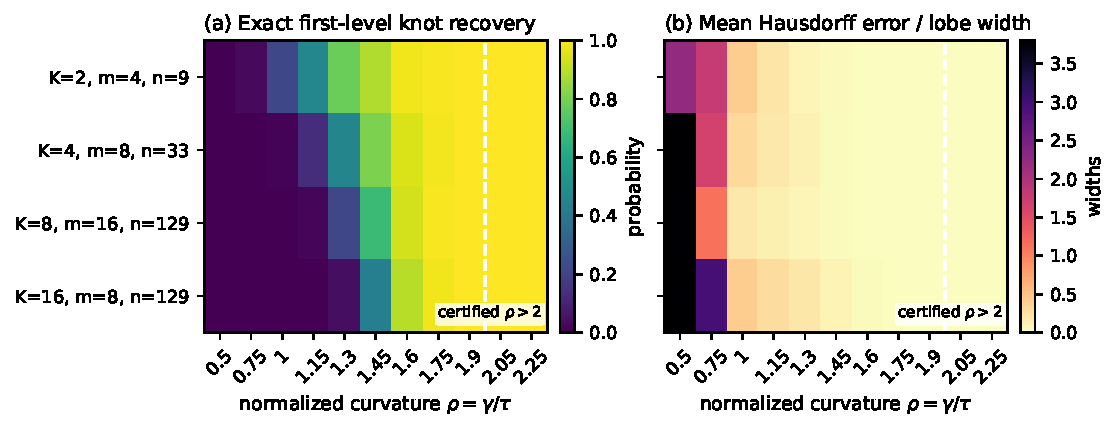
\includegraphics[width=0.98\linewidth]{figures/recovery_phase_diagram.pdf}
\caption{Theorem-linked recovery phase diagram under iid Gaussian noise.
Rows vary lobe count $J$, samples per lobe $m$, and total length $n$; columns
vary normalized active curvature $\rho=\gamma/\tau_\delta$.  Left: exact
first-level knot recovery.  Right: symmetric Hausdorff boundary error divided
by lobe width.  The dashed line marks the strict sufficient region $\rho>2$;
all 8000 draws in that region recovered the exact knots.}
\label{fig:recovery-phase}
\end{figure}


Figure~\ref{fig:approximate-joins} maps departure from exact sampled joins.
The corresponding experiment varied both
$\eta/\tau_\delta$ and $\gamma/\tau_\delta$ over 162,000 independent signals
with unequal adjacent lobe amplitudes.  We compared the noise-only tolerance
$t=\tau_\delta$ with the conservative join-inactivating choice
$t=\eta+\tau_\delta$.  All 72,000 draws in the strict certified region
$\gamma/\tau_\delta>\eta/\tau_\delta+2$ recovered every boundary for both
choices (smallest cellwise 95\% Wilson lower bound 0.9962), with no implication
violation.  Outside that region the noise-only choice was never worse cellwise
and was often markedly better, confirming that $\eta$ is useful for a
certificate but need not be supplied to the algorithm.

\begin{figure}[H]
\centering
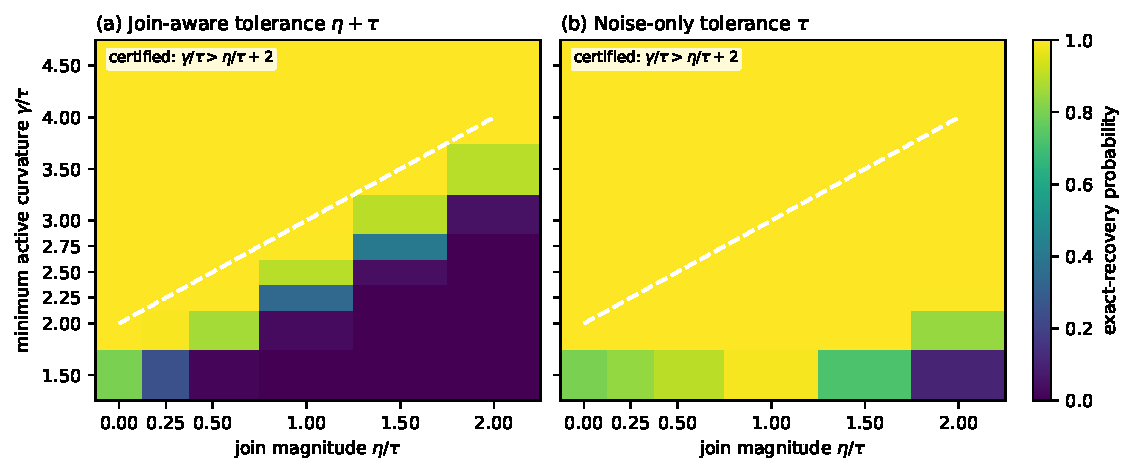
\includegraphics[width=\linewidth]{figures/approximate_join_phase.pdf}
\caption{Departure from exact sampled joins.  Exact first-level recovery is
shown against active curvature and join departure, both normalized by the
simultaneous noise threshold.  The dashed line is the strict sufficient
boundary $\gamma/\tau_\delta>\eta/\tau_\delta+2$.  Left: the conservative
join-inactivating tolerance.  Right: the original noise-only tolerance, which
does not require knowledge of $\eta$.}
\label{fig:approximate-joins}
\end{figure}


\subsection{Synthetic comparisons and computational audit}
On the exact chord-lobe class, centred HCRD recovered the latent chord baseline
exactly and outperformed oracle-tuned EMD, VMD, ITD, trend filtering, CEEMDAN,
and Iterative Filtering baselines.  This class-matched result illustrates the
geometric distinction rather than global dominance over mode decompositions.
With Gaussian noise, a plug-in MAD-thresholded variant retained lower mean
baseline error than the same comparators in fresh-seed confirmations.  Sparse
knot-only storage preserved downstream features bitwise, reduced construction
time 11.89-fold relative to dense materialisation, and independent-signal
process parallelism reached 1.96-fold throughput speedup on 3840 signals.
Complete settings, paired intervals, tables, stable-guide experiments, and the
CWRU ceiling result are reported in the supplement.


\subsection{Expert-labelled chromatographic lobes}
An initial double-group holdout on the expert-labelled EIC corpus of M\"uller
et al. \citep{muller2020eic} gave the largest AP to raw plus HCRD-8 (0.4092 versus
0.3820 for a frozen conventional morphology bank), but the primary two-way
cluster interval crossed zero.  Its ablations showed that the full signed
multilevel decomposition, not polygon area alone, carried the useful signal.
The complete E1 design and table are in the supplement.  The independent E2
study below supplies the central cross-study evidence.

The independent E2 study then used the two fully expert-labelled HILIC studies
of Kumler et al. \citep{kumler2023picky}.  Their two-parameter logistic quality
score combines
correlation with an idealized beta-shaped peak and a residual SNR.  The source
study found this simple model unusually robust under Falkor/MESOSCOPE transfer,
making it a stronger and more interpretable primary comparator than a broad
post-hoc model search.  We used an independent global-window reimplementation
of the published two-component score from the raw mzML feature boxes; on 1495
Falkor features its Pearson
correlations with the authors' SNR and bell-correlation values were 0.906 and
0.789 (Spearman 0.871 and 0.805).

Before reading any raw waveform, we froze both transfer directions, Good versus
Bad labels, exclusion of Ambiguous/standards-only cases, per-file robust
aggregation, one identical standardized logistic learner, and 10,000 paired
feature-bootstrap replicates.  The classifier was fit on all 1821 unambiguous
Falkor features and applied without refitting to 2193 MESOSCOPE features, then
the direction was reversed.  Figure~\ref{fig:lcms-evidence} reports the result.
HCRD-8 plus qscore improved AP over qscore from 0.7774 to 0.8955 in
Falkor-to-MESOSCOPE and from 0.7984 to 0.8990 in the reverse direction.  The
paired differences were 0.1181 ($[0.0613,0.1781]$) and 0.1005
($[0.0559,0.1470]$); both Holm-adjusted values were 0.00040.  Every
pre-specified success criterion was met.

This conclusion was insensitive to four fixed qscore implementations.  We
changed the minimum EIC length from eight to the authors' five-point rule and
tested two-, five-, and seven-variable across-file summaries.  HCRD-8 added
0.0765--0.1517 AP across the resulting eight direction--implementation
contrasts, and every paired 95\% interval remained above zero.  The strongest
qscore-only variants reached AP 0.8107 and 0.8221, while their corresponding
HCRD combinations reached 0.8954 and 0.8986.  On the 1277 unambiguous
author-keyed Falkor features, the current median SNR and correlation summaries
had Pearson correlations 0.934 and 0.867 with the author outputs.  Full
implementation-sensitivity results are in the supplement; the largest
Holm-adjusted bootstrap value across all eight contrasts was 0.0020.

The waveform representations were not equal in width: after fixed per-file
aggregation, qscore had 2 variables, the conventional domain bank 336,
HCRD-1 534, and HCRD-8 2847.  We therefore added a supplementary matched-capacity
control, frozen before its scores were read, that expands the same 75 raw
waveform inputs into Gaussian smoothing, first-derivative, and curvature
channels and aggregates them to exactly 2847 variables.  Its result is
reported separately below because it was not part of the pre-specified E2
family.

Multilevel HCRD also exceeded one-level HCRD in both directions, by 0.0439 and
0.0544 AP; the second interval $[0.0076,0.0955]$ remained positive after Holm
correction ($p=0.0372$), while the first $[-0.0167,0.1060]$ did not.  The best
point representation was HCRD scalar geometry plus qscore (AP 0.9150) in the
first direction and the multilevel area/energy spectrum plus qscore (0.9412) in
the second.  Conversely, full HCRD-8 did not establish a difference from the
larger conventional domain bank: its two intervals were
$[-0.0469,0.0561]$ and $[-0.0479,0.0154]$.  Thus E2 confirms incremental
multilevel convex-lobe information over the established minimal score, while
the optimal compression of that hierarchy and superiority to every non-neural
domain representation remain open.

The primary E2 bootstrap is conditional on the fitted source-study model.
We therefore added two fixed secondary sensitivities.  The first keeps the
source model fixed and resamples target retention-time blocks, directly
testing the conditional transfer estimand under local feature dependence.  At
the primary 60-second width, HCRD-8+Q minus qscore remained positive in both
directions: 0.1181 ($[0.0130,0.2190]$) and 0.1005
($[0.0338,0.1965]$).  Both 30-second intervals were also positive; only the
Falkor-to-MESOSCOPE interval crossed zero at the coarsest 120-second width.
The second sensitivity resamples source and target blocks, refits the source
learner in every replicate, and varies block width from 30 to 120 seconds.  A
separate ten-fold
acquisition-file deletion recomputes the per-file representation aggregates
before refitting both directions.  These analyses propagate source-model,
local retention-time, and acquisition-file sensitivity, but the public schema
contains no compound/adduct identifiers and cannot support a chemical-cluster
bootstrap.

\ifdefined\SPsubmission
\IfFileExists{../generated/e2_refit_sensitivity_table.tex}{\begin{table}[H]
\centering
\caption{E2 dependence and refitting sensitivity for HCRD-8+Q minus qscore AP. Fixed-source rows report the original point difference and target RT-block percentile interval; source-refit rows give the bootstrap mean and interval. The file row gives the range across ten delete-group representation-and-model refits.}
\label{tab:e2-refit-sensitivity}
\small
\resizebox{\linewidth}{!}{%
\begin{tabular}{lcc}
\toprule
Design & Falkor $\to$ MESOSCOPE & MESOSCOPE $\to$ Falkor \\
\midrule
Fixed-source target RT blocks (30 s) & 0.1181 [0.0340, 0.2051] & 0.1005 [0.0402, 0.1762] \\
Fixed-source target RT blocks (60 s) & 0.1181 [0.0130, 0.2190] & 0.1005 [0.0338, 0.1965] \\
Fixed-source target RT blocks (120 s) & 0.1181 [-0.0227, 0.2418] & 0.1005 [0.0415, 0.2082] \\
\midrule
Source-refit RT blocks (30 s) & 0.1087 [-0.0105, 0.2074] & 0.0556 [-0.0671, 0.1602] \\
Source-refit RT blocks (60 s) & 0.1000 [-0.0444, 0.2179] & 0.0515 [-0.0935, 0.1742] \\
Source-refit RT blocks (120 s) & 0.0886 [-0.1514, 0.2508] & 0.0574 [-0.0803, 0.1761] \\
Acquisition-file delete-group & 0.1030--0.1397 (10/10 positive) & 0.0517--0.1058 (10/10 positive) \\
\bottomrule
\end{tabular}
}
\end{table}
}{}
\else
\IfFileExists{generated/e2_refit_sensitivity_table.tex}{\begin{table}[H]
\centering
\caption{E2 dependence and refitting sensitivity for HCRD-8+Q minus qscore AP. Fixed-source rows report the original point difference and target RT-block percentile interval; source-refit rows give the bootstrap mean and interval. The file row gives the range across ten delete-group representation-and-model refits.}
\label{tab:e2-refit-sensitivity}
\small
\resizebox{\linewidth}{!}{%
\begin{tabular}{lcc}
\toprule
Design & Falkor $\to$ MESOSCOPE & MESOSCOPE $\to$ Falkor \\
\midrule
Fixed-source target RT blocks (30 s) & 0.1181 [0.0340, 0.2051] & 0.1005 [0.0402, 0.1762] \\
Fixed-source target RT blocks (60 s) & 0.1181 [0.0130, 0.2190] & 0.1005 [0.0338, 0.1965] \\
Fixed-source target RT blocks (120 s) & 0.1181 [-0.0227, 0.2418] & 0.1005 [0.0415, 0.2082] \\
\midrule
Source-refit RT blocks (30 s) & 0.1087 [-0.0105, 0.2074] & 0.0556 [-0.0671, 0.1602] \\
Source-refit RT blocks (60 s) & 0.1000 [-0.0444, 0.2179] & 0.0515 [-0.0935, 0.1742] \\
Source-refit RT blocks (120 s) & 0.0886 [-0.1514, 0.2508] & 0.0574 [-0.0803, 0.1761] \\
Acquisition-file delete-group & 0.1030--0.1397 (10/10 positive) & 0.0517--0.1058 (10/10 positive) \\
\bottomrule
\end{tabular}
}
\end{table}
}{}
\fi

The source-refit mean remained positive in all six direction--block-width
designs (positive paired replicates: 80.7--96.3\%), but every percentile
interval crossed zero.  This secondary analysis therefore preserves the sign
of the point effect without establishing it after source-model and RT-block
resampling.  The stronger file-deletion check was uniformly positive: the
full-pipeline difference ranged from 0.1030 to 0.1397 in
Falkor-to-MESOSCOPE and from 0.0517 to 0.1058 in the reverse direction over
all 20 direction--fold fits.

In the matched-capacity sensitivity analysis, the Gaussian-derivative control
had AP 0.9063 versus 0.8955 for HCRD-8 in Falkor-to-MESOSCOPE; the HCRD minus
control difference was $-0.0108$ ($[-0.0594,0.0405]$, Holm-adjusted
$p=0.7653$).  In the reverse transfer, HCRD-8 had AP 0.8990 versus 0.7815, a
difference of 0.1175 ($[0.0624,0.1654]$, adjusted $p=0.00040$).  Thus raw
dimensionality does not explain the reverse-direction gain, but the first
direction provides no evidence that HCRD uniformly dominates a comparably
rich conventional scale-space bank.

\begin{figure}[H]
\centering

\includegraphics[width=\linewidth]{figures/lcms_evidence.pdf}
\caption{Independent expert-labelled LC--MS evidence.  Panel a shows average
precision for the first double holdout and both no-refit E2 transfers; ``raw /
qscore'' denotes the task-appropriate minimal representation.  Panel b shows
the predeclared HCRD-8 difference from the primary comparator.  The E1 interval
resamples both sample and candidate-ion groups; E2 target-feature intervals are
conditional on the trained source models.  F and M abbreviate Falkor and
MESOSCOPE.}
\label{fig:lcms-evidence}
\end{figure}

\ifdefined\SPsubmission
\paragraph{External application boundaries.}
On the conditionally labelled Pttime subset, HCRD-8+Q achieved residual-error
AP 0.5085 versus 0.0391 for qscore and retrieved 7 of 17 bad cases within the
top 5\% review queue, compared with none for qscore.  This is a conditional
reranking result, not a full-cohort estimate.  Under the larger TARDIS/FAME
laboratory shift, the HCRD-8+Q gain over qscore was 0.0725 but its interval
$[-0.0155,0.1345]$ crossed zero; HCRD-8 also tied HCRD-1 and a compact
conventional bank was point-best.  Additional LC--MS, ECG, PPG, anomaly,
classification, and prognostic boundary studies are reported in the
supplement.  Collectively they delimit the supported setting to pre-bounded
compact-lobe curation rather than generic signal decomposition.
\else
LCMS-E5 tested a different operational consequence on Pttime.  The source
authors manually labelled only 400 of 7781 features: those already assigned a
probability above 0.9 by their two-variable model.  We therefore froze E5 as a
conditional residual-error reranking test, not as a third fully labelled
cohort.  Before any target waveform was inspected, HCRD-8, the learner,
AP-bad endpoint, and success rule were fixed.  The Falkor and MESOSCOPE cases
were pooled for training and the model was applied without refitting to the 365
unambiguous Pttime cases (348 Good, 17 Bad).  Archive inspection before feature
extraction revealed both ion modes; the source pipeline's POS filename schema
fixed the compatible 52 positive-mode files, and this correction was recorded
before any E5 score was computed.

Table~\ref{tab:lcms-e5} shows that HCRD-8 passed both pre-specified conditions.
It attained AP-bad 0.5085 versus 0.0391 for qscore, a difference of 0.4694 with
a paired class-stratified bootstrap interval $[0.2489,0.6762]$
($p=0.00020$), and exceeded HCRD-1 by 0.2240
($[0.0707,0.3544]$, $p=0.00060$).  Seven of the 17 residual bad features were
placed in the top 19 (5\%) review positions, versus none under qscore.  At
1\%, 5\%, and 10\% queue budgets (4, 19, and 37 reviews), HCRD-8 retrieved
4, 7, and 8 bad cases, respectively, versus 0, 0, and 1 for qscore.  Hence its
5\%-budget precision was 36.8\% and residual-bad recall was 41.2\%.  To reach
at least 50\% recall (9/17), HCRD-8 required 44 reviews versus 284 under
qscore, an 84.5\% workload reduction at the same integer recall target.  HCRD-8
also had the best point estimate, but its 0.1212 AP advantage over DOMAIN+Q was
not established ($[-0.0100,0.2794]$, $p=0.0818$).  Thus E5 confirms practical
conditional triage value and the need for multiple levels; selection of the
labelled population prevents claims about all 7781 Pttime features, recall,
calibration, or FDR.

\begin{table}[H]
\centering
\caption{Frozen E5 Pttime residual-bad reranking within the 365 unambiguous
source-model-selected features.  AP-bad is primary; queue entries give bad
features retrieved among 17 at review budgets of 4, 19, and 37 cases.}
\label{tab:lcms-e5}
\begin{tabular}{lrrrrr}
\toprule
Representation & AP-bad & ROC AUC-bad & 1\% & 5\% & 10\% \\
\midrule
qscore & 0.0391 & 0.3403 & 0 & 0 & 1 \\
DOMAIN+Q & 0.3873 & 0.8115 & 4 & 6 & 6 \\
HCRD-1+Q & 0.2845 & 0.7792 & 2 & 5 & 7 \\
HCRD-8+Q & \textbf{0.5085} & \textbf{0.8646} & \textbf{4} & \textbf{7} & \textbf{8} \\
HCRD geometry+Q & 0.3540 & 0.8081 & 3 & 6 & 7 \\
Area/energy+Q & 0.1367 & 0.7194 & 1 & 3 & 5 \\
\bottomrule
\end{tabular}
\end{table}

E6 then tested a more severe external shift using the manually rated TARDIS
FAME saliva panel \citep{vangeenderhuysen2025tardis}.  The protocol, primary
cohort, representations, pooled Falkor+MESOSCOPE learner, AP-bad endpoint, two
co-primary comparisons, 20,000-replicate paired bootstrap, and seed were frozen
before any rating row was inspected.  The 5.67-GB Zenodo archive matched its
published MD5.  A pre-score availability audit found 119 positive-polarity QC
mzXML files but no numerical negative-polarity EICs; the positive stratum was
therefore evaluated and the negative stratum declared unavailable rather than
approximated from diagnostic images.  Fixed 10-ppm, 60-s boxes yielded valid
feature banks for all 212 keyed positive targets, with median QC availability
0.9412; 108 Good and 84 Bad targets entered the binary endpoint and 20
Ambiguous targets only the ordered-label sensitivity analysis.

Table~\ref{tab:lcms-e6} reports the no-refit result.  HCRD-8+Q improved AP-bad
over qscore by 0.0725, but the percentile interval $[-0.0155,0.1345]$ crossed
zero ($p=0.1115$), so the first co-primary rule failed.  It was tied with
HCRD-1+Q (difference $-0.0016$, $[-0.0500,0.0453]$), so the second also failed.
DOMAIN+Q had the largest AP point estimate, while HCRD geometry+Q had the
largest ROC AUC.  Thus decomposition-derived shape information transferred in
point estimate beyond qscore, but E6 does not establish that eight levels are
needed or that HCRD beats a compact conventional domain bank under this
acquisition and processing shift.

\begin{table}[H]
\centering
\caption{Frozen E6 no-refit transfer to 192 unambiguous positive-polarity
TARDIS/FAME targets.  AP-bad is primary; enrichment is the Bad fraction in the
top score decile divided by overall Bad prevalence.}
\label{tab:lcms-e6}
\begin{tabular}{lrrr}
\toprule
Representation & AP-bad & ROC AUC-bad & Top-decile enrich. \\
\midrule
qscore & 0.4353 & 0.5230 & 0.686 \\
DOMAIN+Q & \textbf{0.5193} & 0.6030 & 1.257 \\
HCRD-1+Q & 0.5094 & 0.5902 & \textbf{1.486} \\
HCRD-8+Q & 0.5078 & 0.5998 & 1.371 \\
HCRD geometry+Q & 0.5044 & \textbf{0.6049} & \textbf{1.486} \\
Area/energy+Q & 0.3847 & 0.4377 & 0.571 \\
\bottomrule
\end{tabular}
\end{table}


Two LC--MS boundary tests and five cross-domain searches delimit the claim.
HCRD did not improve a morphology-saturated TargetedMSQC bank, and sign-aware
lower-envelope estimators were better for chromatographic baseline recovery.
It also did not establish superiority for specialist ECG/PPG delineation,
bearing classification at ceiling, or real-KPI anomaly detection; full tables
and the stability/persistence audits are in the supplement.  These results
support the narrower use of HCRD as a transparent representation for already
bounded compact-lobe morphology.
Figure~\ref{fig:falsification} illustrates the complementary curvature-
visibility failure behind one of these boundaries.

\begin{figure}[H]
\centering
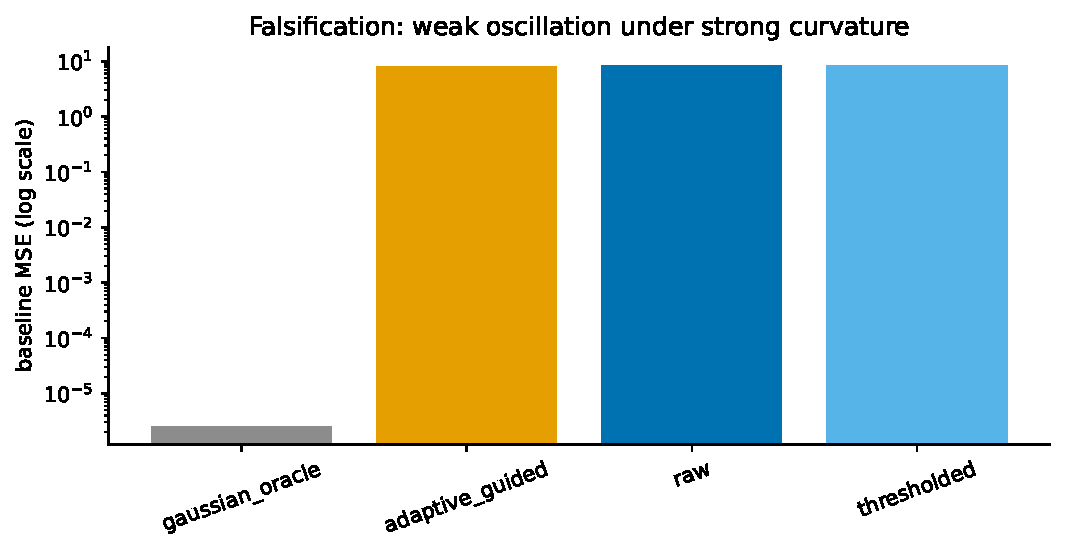
\includegraphics[width=0.92\linewidth]{figures/curvature_visibility_failure.pdf}
\caption{Limitation under strong background curvature. When background
curvature exceeds the oscillatory curvature, raw HCRD cannot expose the
oscillation and its chord baseline is inappropriate.}
\label{fig:falsification}
\end{figure}
\fi

\section{Discussion}
HCRD occupies a specific rather than universal signal-processing niche.  Its
algorithmic appeal is its economy: divided-slope comparisons select maximal
one-sign runs, endpoint chords form the next baseline, and subtraction gives
an exactly reconstructing hierarchy.  The resulting lobes expose support,
sign, amplitude, residual shape, area, and level without a learned dictionary
or a continuous smoothing parameter.  This combination of simplicity and
interpretability is the main contribution; its intended use is as a geometric
representation of bounded waveform morphology, not as a replacement for every
task-specific detector or decomposition.

The generative recovery result makes that niche testable.  On alternating
one-sign curvature blocks, the same geometry used by the algorithm yields
exact first-level boundary recovery and explicit component-error control.  The
condition $\gamma>\eta+2\tau_\delta$ allows nonzero sampled join curvature;
the original noise-only threshold remains valid and does not require $\eta$.
Across the exact- and approximate-join phase experiments, zero failures were
observed among 80,000 draws in the strict certified regions.  Outside the sufficient
boundary, the less conservative noise-only threshold was often more accurate.
This is a class-specific mechanism result, not a separation theorem against
every adaptive representation.

The clearest practical evidence is expert curation of pre-bounded LC--MS
features.  In the two frozen no-refit E2 transfers, multilevel HCRD improved
average precision over an independent reimplementation of the published
two-component score by 0.1181 and 0.1005, with
Holm-adjusted $p=0.00040$ in both directions.  HCRD-8 had positive point
differences from the one-level variant in both transfers, with
multiplicity-adjusted support in one.  The equal-dimensional conventional
control tied HCRD-8 in one transfer, whereas HCRD-8 was superior in the
reverse.  The incremental gain also survived four qscore implementations in
both directions, so imperfect reproduction of one two-variable comparator is
not an adequate explanation.  It remained positive in all 20 direction--fold
comparisons after acquisition-file deletion and full representation refitting.
Fixed-source target RT-block intervals were positive in both directions at the
primary 60-second width, so the conditional result is not an artefact of
independent target-feature resampling.  Source-refit RT-block means were also
positive for all tested block widths, although their percentile intervals
included zero.  Hence the E2 claim remains conditional on the fitted source
models rather than an unconditional population-level assertion.
E5 further supports residual-error reranking when only conditional
labels are available.  E6, however, did not confirm superiority under the
larger TARDIS/FAME laboratory shift: the gain over qscore was 0.0725 only in
point estimate, HCRD-8 tied HCRD-1, and a compact conventional feature bank
remained best.  Thus the evidence supports transferable value for
pre-bounded compact-lobe curation, with hierarchy depth still dependent on the
acquisition domain.

Results outside pre-bounded compact-lobe curation sharpen that positioning.
HCRD added no benefit after a morphology-saturated LC--MS feature bank (E3), and
sign-specific lower-envelope estimators were better chromatographic baseline
models (E4).  The ECG-specific \texttt{ecgpuwave} system retained lower QTDB
boundary error; tuned \texttt{find\_peaks} remained better overall on wearable
PPG; and the supervised UCR, real WSD/AIOps anomaly, and bearing-RUL studies did
not establish an advantage.  These are important boundaries rather than a
contradiction: a small generic geometry should not be expected to dominate
specialist multichannel morphology rules, correct sign priors, or large
supervised representations on their native objectives.

The empirical and theoretical results together suggest a practical selection
rule.  HCRD is most plausible when the object is already bounded, an endpoint
chord is a meaningful local reference, and scientifically relevant structure
appears as signed convex or concave excursions whose complete hierarchy may
matter.  It is less well matched to frequency separation, instantaneous
frequency estimation, weak oscillations on a strongly curved trend, or noisy
samplewise decisions without thresholding.  Polygon mass and its levelwise
time series are inexpensive auxiliary summaries, but the PPG and RUL evidence
does not support replacing the full decomposition by area alone.

The simplicity also has computational consequences.  With sparse retained
knots and the halving property, total hierarchy work is linear in signal
length; dense materialization can remain $O(n\log n)$.  On P2R the knot-only
implementation was 11.89-fold faster than dense materialization while
preserving knots and downstream features bitwise.  Independent signals admit
exact process parallelism, including a 1.96-fold median speedup on the
3840-signal sparse P3 batch.  Absolute speedups remain hardware- and
batch-dependent, and the present Python implementation does not establish an
optimal systems realization.

The theory states the same boundary precisely.  A hard knot map cannot be
globally continuous while preserving every generic raw branch decision
(Theorem~\ref{thm:impossibility}); persistence matching and the proximal outer
split provide well-posed stable alternatives, while deterministic and
stochastic margins certify local hard-HCRD decisions.  The explicit
chord-lobe theorem turns those decision margins into boundary and component
recovery on a declared generative class.  Optional rank-aware scans and
independent-guide inference in the supplement provide calibrated uses of the
resulting shapes.  These results justify a signed curvature-lobe
representation, but do not identify its details with intrinsic modes.

The remaining gaps are consequently focused.  The theory still assumes known
or conservatively supplied noise scale and, for optional inference results,
covariance, dependence lag, and stability radius.  Estimated versions,
infinite-memory noise, unsampled transitions with quantitative localisation,
and general polygonal templates remain open.  A minimax separation from
all competing adaptive dictionaries is not claimed.  Empirically,
representation selection must be frozen
outside E2, and a further waveform-backed cross-laboratory LC--MS cohort is
needed to resolve the roughly 0.07 AP effect seen in E6 and determine when
multilevel depth transfers.  The present evidence therefore supports a
task-specific method with unusually transparent mechanics and failure modes.
Broader state-of-the-art performance requires future independent confirmation.

\section*{Code and data availability}
Implementation, tests, protocols, compact outputs, hashes, and environment
instructions are at \url{https://github.com/Safreliy/hcrd}. Large derived
caches are rebuilt locally. Code: MIT; manuscript, documentation, original
figures, protocols, and results: CC BY 4.0.

\section*{CRediT authorship contribution statement}
Saveliy Baturin: Conceptualization; Methodology; Software; Validation; Formal
analysis; Investigation; Data curation; Visualization; Project administration.
Writing--original draft; Writing--review and editing.

\section*{Funding}
This research received no specific grant from funding agencies in the public,
commercial, or not-for-profit sectors.

\section*{Declaration of competing interest}
The author declares no competing financial interests or personal relationships
that could have influenced the work reported in this article.

\section*{Declaration of generative AI and AI-assisted technologies in the manuscript preparation process}
During the preparation of this work, the author used OpenAI Codex to assist
with literature organization, language and clarity editing, and manuscript
formatting.  After using this tool, the author reviewed and edited the content
as needed and takes full responsibility for the content of the published
article.

\footnotesize
\setlength{\bibsep}{1pt}
\ifdefined\SPsubmission
\bibliographystyle{elsarticle-num}
\bibliography{../references}
\else
\bibliographystyle{plainnat}
\bibliography{references}
\fi
\end{document}
